\subsection{Statistische Gemische und Dichtematrix}
	Beispiel: Wir wissen, dass ein System mit einer Wahrscheinlichkeit $W_1$ sich in einem quantenmechanischen Zustand $\ket{\psi_1}$ und $W_2$ in $\ket{\psi_2}$ etc. befindet.
	
	Man nennt dies ein statistisches Gemisch:
		\begin{align*}
			(\ket{\psi_1}, \ket{\psi_2}, \ldots; W_1, W_2, \ldots) \text{ mit } \sum_d W_{d} = 1.
		\end{align*}
	Die $W_d$ sind \underline{klassische} Wahrscheinlichkeiten, die additiv sind. 
	
	Sie haben ihren Ursprung z.B. in nicht-perfekten Instrumenten bei der Präsentation eines Zustands
	$\Rightarrow$ von Regel \ref{Regel3}.
	\subsubsection*{Stern-Gerlach Experiment}
		\begin{figure} [h]
			\begin{center}
				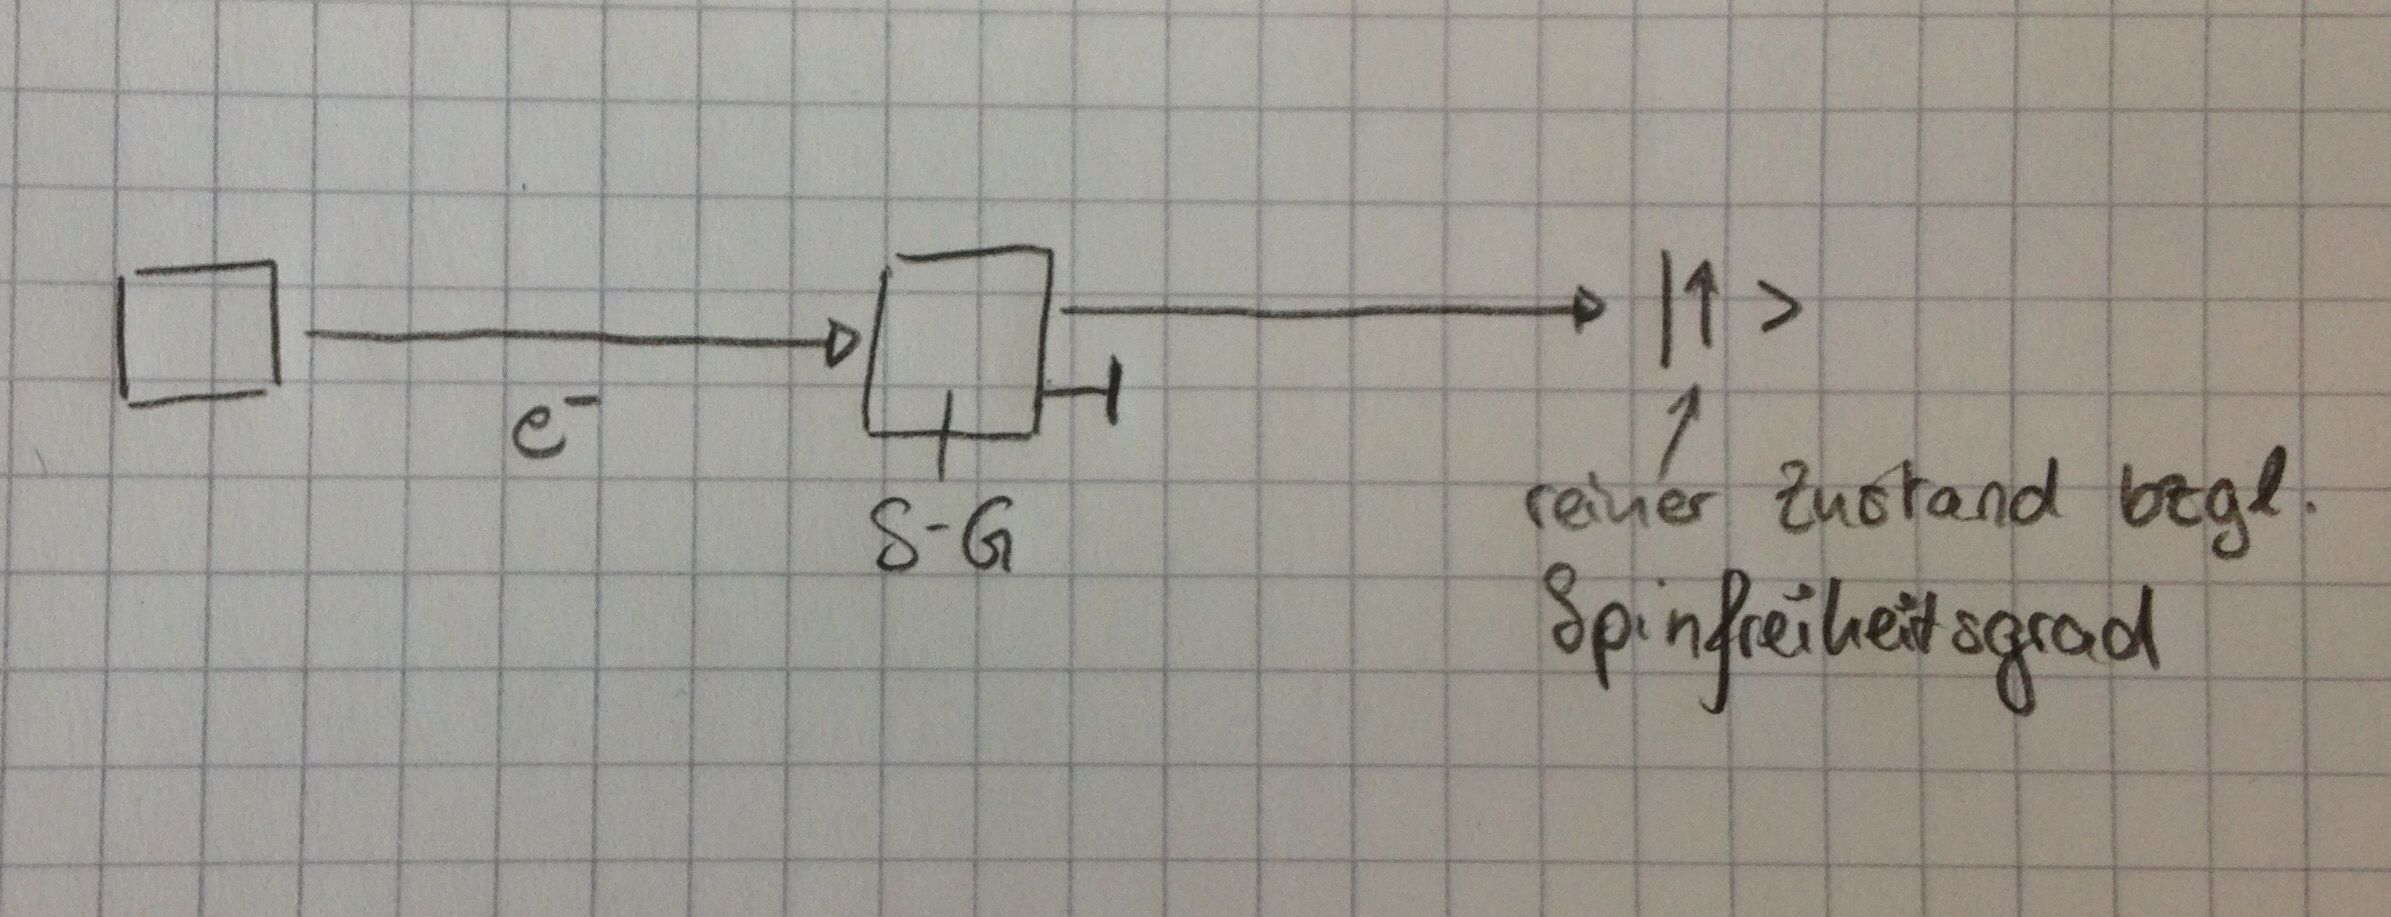
\includegraphics[width=0.7\textwidth]{Statistische_Gemische_und_Dichtematrix1}
			\end{center}
		\end{figure}
	Was ist mit Gemischen?
	\begin{align*}
		\alpha \ket{\uparrow} &+ \beta \ket{\downarrow},& \alpha^2 + \beta^2 &= 1 \\
		W_\uparrow\ket{\uparrow} &+ W_\downarrow \ket{\downarrow},& W_\uparrow + W_\downarrow &= 1.
	\end{align*}
	\begin{align*}
		W(A = a_n; \ket{\psi}) &= \braket{\psi | \hat{P}_n | \psi} \\
		\rho &\coloneqq (\ket{\psi_1}, \ket{\psi_2}, \ldots; W_1, W_2, \ldots) \\
		W(A=a_m; \rho) &= \sum_{d} W_d (A = a_m ; \ket{\psi_d}) \\
		&= \sum_d W_d \braket{\psi_d | \hat{P_n} | \psi_d} 
	\end{align*}
	Grundannahme: quantenmechanische und klassische Wahrscheinlichkeiten sind unkorreliert
	
	Basis $\{\ket{e_1}, \ket{e_2}, \ldots \}$ von $\Hil$
		\begin{align*}
			\mathrm{Sp}\, \hat{B} &\coloneqq \sum_i \braket{e_i | \hat{B} | e_i} &
			\sum_i \ket{e_i} \bra{e_i} &= \mathds{1} \\
			\braket{\psi| \hat{B} | \psi} &= 
			\sum_i \braket{\psi | \hat{B} | e_i} \braket{e_i | \psi} \\
			&= \sum_i \braket{e_i | \psi} \braket{\psi | \hat{B} | e_i} \\
			&= \mathrm{Sp}\,(\ket{\psi} \bra{\psi} \hat{B}) \\
			&= \mathrm{Sp}\, (\hat{P}_{\ket{\psi}} \hat{B}) &
			\text{mit } \hat{P}_{\ket{\psi}} &= \ket{\psi} \bra{\psi} 
		\end{align*}
	$\hat{P}^2_{\ket{\psi}} =\hat{P}_{\ket{\psi}}$ weil $\braket{\psi | \psi} = 1$
	
	Analog:
		\begin{align*}
			W(A = a_n; \ket{\psi}) &= \braket{\psi | \hat{P}_n | \psi} = 
			\mathrm{Sp } \hat{P}_{\ket{\psi}} \hat{P}_n \\
			\erw{A}_\psi &= \mathrm{Sp} \, (\hat{P}_{\ket{\psi}}, \hat{A}) 
		\end{align*}
	Dichte - ``Matrix'':
		\begin{align*}
			\boxed{
					\hat{\rho} \coloneqq \sum_d W_d \hat{P}_{\ket{\psi_d}} = 
					\sum_d W_d \ket{\psi_d} \bra{\psi_d}
				}
		\end{align*}
		\begin{align*}
			W(A = a_n; \rho) &= \sum_d W_d \mathrm{Sp}\, (\hat{P}_{\ket{\psi_d}} \hat{P}_n) \\
			&= \mathrm{Sp}\, \left(
				\left(
					\sum_d W_d \hat{P}_{\ket{\psi_d}} 
				\right) \hat{P}_n
			\right)
		\end{align*}
	Wahrscheinlichkeit bei Messung von $A$ auf Gemisch $\rho$ das Ergebnis $a_n$ zu finden:
		\begin{empheq}[box = \boxed]{align*}
			W(A = a_n; \rho) &= \mathrm{Sp} \, (\hat{\rho} \hat{P}_n)\\
			\erw{A}_\rho = \mathrm{Sp}\, (\hat{\rho} \cdot \hat{A}) 
		\end{empheq}	
		\begin{align*}
			\mathrm{Sp}\, \hat{\rho} &= \sum_d W_d = 1 \\
			\mathrm{Sp}\, (\hat{\rho}^2) &\leq 1
		\end{align*}
	Eigenschaften der Dichtematrix eines Gemisches $\rho$:
		\begin{enumerate}[1.]
			\item $\hat{\rho} = \hat{\rho}^\dagger$
			\item $\braket{\psi | \hat{\rho} | \psi} \geq 0 ~\text{für alle} \ket{\psi} \in \Hil$ 
			\item $\mathrm{Sp}\, \hat{\rho} =1$.
			\item $\mathrm{Sp}\, \hat{\rho}^2 \leq 1, ~
			\mathrm{Sp}\,\hat{\rho}^2 \Leftrightarrow \rho$ ist ein Reiner Zustand
		\end{enumerate}
	Beispiel
		\begin{align*}
			S_z &= \frac{\hbar}{2} \sigma_z =
			\begin{pmatrix}
				1 & 0 \\
				0 & -1
			\end{pmatrix} ,&
			S_x &= \frac{\hbar}{2} 
			\begin{pmatrix}
				0 & 1 \\
				1 & 0 
			\end{pmatrix} \\
			&\text{EV} : 
			\begin{pmatrix}
			1 \\
			0 
			\end{pmatrix},
			\begin{pmatrix}
			0 \\
			1
			\end{pmatrix} 
			& &\frac{1}{\sqrt{2}}
			\begin{pmatrix}
			1 \\
			1 
			\end{pmatrix} ,
			\frac{1}{\sqrt{2}}
			\begin{pmatrix}
			1 \\
			-1
			\end{pmatrix} \\
			\hat{P}_{S_z = \frac{\hbar}{2}} &=
			\begin{pmatrix}
			1 \\
			0
			\end{pmatrix} 
			\begin{pmatrix}
			1 & 0
			\end{pmatrix} =
			\begin{pmatrix}
			1 & 0 \\
			0 & 0
			\end{pmatrix}, &
			\hat{P}_{S_z = -\frac{\hbar}{2}} &= 
			\begin{pmatrix}
				0 & 0 \\
				0 & 1
			\end{pmatrix} \\
			\hat{P}_{S_x = \frac{\hbar}{2}} &= 
			\frac{1}{2} 
			\begin{pmatrix}
				1 \\
				1
			\end{pmatrix} 
			\begin{pmatrix}
			1 & 1
			\end{pmatrix}
			= \frac{1}{2} 
			\begin{pmatrix}
			1 & 1 \\
			1 & 1
			\end{pmatrix}, &
			\hat{P}_{S_x = -\frac{\hbar}{2}} &=
			\frac{1}{2} 
			\begin{pmatrix}
				1 & - 1 \\
				-1 & 1 
			\end{pmatrix}
		\end{align*}
	Dichtematrix
		\begin{align*}
			\hat{\rho} &\coloneqq \frac{1}{2}
			\begin{pmatrix}
			1 & 0 \\
			0 & 1
			\end{pmatrix}
			~ \mathrm{Sp}\, \hat{\rho} = 1 \checkmark \\
			\hat{\rho}^2 &= \frac{1}{4} 
			\begin{pmatrix}
				1 & 0 \\
				0 & 1
			\end{pmatrix}
			\Rightarrow \mathrm{Sp}\, \hat{\rho}^2 = \frac{1}{2} \Rightarrow \text{Gemisch} \\
			\hat{\rho} &= \frac{1}{2} 
			\left(
				\hat{P}_{S_z = \frac{\hbar}{2}} + \hat{P}_{S_z = -\frac{\hbar}{2}}
			\right) =
			\frac{1}{2}
			\left(
				\hat{P}_{S_x = \frac{\hbar}{2}} + \hat{P}_{S_x = -\frac{\hbar}{2}}
			\right) \\
			&= \frac{\alpha}{2}
			\left(
			\hat{P}_{S_z = \frac{\hbar}{2}} + \hat{P}_{S_z = -\frac{\hbar}{2}}
			\right) +
			\frac{1 - \alpha}{2}
			\left(
			\hat{P}_{S_x = \frac{\hbar}{2}} + \hat{P}_{S_x = -\frac{\hbar}{2}}
			\right)
		\end{align*}
	Zerlegung der Dichtematrix nach reinen Zuständen ist nicht eindeutig.
	
	$\{\hat{\rho}_1, \ldots, \hat{\rho}_k\}:$ Dichtematrizen, $\{r_1, \ldots, r_k\}$ positive reelle Zahlen mit $(\sum_{k = 1}^{K} r_k = 1) ~\sum_{k = 1}^{K} r_k \hat{\rho}_k$ ist Dichtematrix, weil 
	
	$\mathrm{Sp}\, (\sum_k r_k \hat{\rho}_k) = 1 \Rightarrow$ Menge aller Dichtematrizen ist konvex.
	
	Lediglich Dichtematrizen reiner Zustände $\hat{P}_{\ket{\psi}} = \ket{\psi} \bra{\psi}$ lassen sich nicht weiter zerlegen.
	
	Vorgriff auf statistische Physik: Thermisches Gemisch
		\begin{align*}
			\hat{\rho}_T &= \frac{e^{-\beta \hat{H}}}{Z (\beta)} ,&
			\beta &= \frac{1}{k T},&
			T&: \text{Temperatur} 
		\end{align*}
	Zustandssumme: 
		\begin{align*}
			Z(\beta) = \mathrm{Sp}\, e^{-\beta \hat{H}} 
			&= \sum_n \braket{E_n | e^{-\beta H} | E_n} \\
			&= \sum_n e^{-\beta E_n} \braket{E_n | E_n} \\
			&= \sum_n e^{-\beta E_n}
		\Rightarrow \mathrm{Sp}\, \hat{\rho}_T = 1 \\
		\hat{\rho}_T &= \sum_n \frac{e^{-\beta E_n}}{Z (\beta)} \ket{E_n} \bra{E_n}
		\end{align*}

	Bsp: $\{\ket{\uparrow}, \ket{\downarrow} \}$ mit Wahrheitswerten $W_1, W_2$ 
		\begin{align*}
			\hat{\rho} &= W_\uparrow \hat{P}_\uparrow + W_\downarrow \hat{P}_\downarrow =
			\begin{pmatrix}
				W_\uparrow & 0 \\
				0 & W_\downarrow 
			\end{pmatrix}&
			\sigma_z &= 
			\begin{pmatrix}
				1 & 0 \\
				0 & -1
			\end{pmatrix} \\
			\erw{S_z} \rho &= 
			\frac{\hbar}{2} \mathrm{Sp}\, (\hat{\rho} \sigma_z) =
			\frac{\hbar}{2} \mathrm{Sp}\, 
			\begin{pmatrix}
			W_\uparrow & 0 \\
			0 & W_\downarrow 
			\end{pmatrix} =
			\frac{\hbar}{2} (W_\uparrow - W_\downarrow) 
		\end{align*}
	Spezialfall: $W_\uparrow = W_\downarrow = \frac{1}{2}$ Isotropes Gemisch $\erw{S_z} = 0$
	\\
	Spezialfall 2: $W_\uparrow = 1, W_\downarrow = 0$ reiner Zustand $\erw{S_z}_{\ket{\uparrow}} = \frac{\hbar}{2}$
	
	Reiner Zustand $\ket{\psi}$ \marginpar{11.01.16} \\
	Projektor auf reinem Zustand $ \hat{P}_{\ket{\psi}} = \ket{\psi} \bra{\psi}$ \\
	Projektor auf UR von Eigenzuständen von $\hat{A}$ mit EW $a_m$ : 
	$\hat{P}_m = \sum_{j = 1}^{d(j)} \ket{a_m, j} \bra{a_m, j}$ \\
	Dichteoperator/matrix (statistischer Operator) : $\hat{\rho}$ \\
	reiner Zustand: $\hat{\rho} = \ket{\psi} \bra{\psi} = \hat{P}_{\ket{\psi}}$,
	$\hat{\rho}^2 = \hat{\rho} , \mathrm{Sp} \hat{\rho}^2 = 1$ (Sp $\hat{\rho} = 1$ immer)\\
	Gemischter Zustand: $\hat{\rho} = \sum_d W_d \ket{\psi_d} \bra{\psi_d}$ \\
	Siehe oben
	
	Anderes Beispiel:
	
	Reiner Zustand
		\begin{align*}
			\ket{\phi} &= \frac{1}{\sqrt{2}} \left(
				\ket{\uparrow} + e^{i\phi} \ket{\downarrow}
			\right) = \frac{1}{\sqrt{2}} 
			\begin{pmatrix}
				1 \\
				e^{i\phi}
			\end{pmatrix}
		\end{align*}
	Eigenwerte von $\hat{S}_{\vec{e}}$ mit $\vec{e} = (\cos\phi , \sin \phi, 0)$
	$(\hat{S}_{\vec{e}} = \vec{S} \cdot \vec{e}) : \pm \frac{\hbar}{2}$ \\
	Eigenzustand von $\hat{S}_{\vec{e}}$ mit Eigenwert $+ \frac{\hbar}{2}$ 
		\begin{align*}
			\hat{S}_{\vec{e}} &= 
			\frac{\hbar}{2} \left(
				\cos \phi \sigma_x + \sin \phi \sigma_y 
			\right) = 
			\frac{\hbar}{2}
			\left. 
			\begin{pmatrix}
				0 & e^{i\phi} \\
				e^{i\phi} & 0 
			\end{pmatrix}
			\right| 
			\text{Test: }
			\begin{pmatrix}
				-1 & e^{i\phi} \\
				e^{i\phi} & -1
			\end{pmatrix}
			\begin{pmatrix}
			1 \\
			e^{i\phi}
			\end{pmatrix}
			= 0 \checkmark
		\end{align*}
		\begin{align*}
			\hat{\rho}_\phi &= \hat{P}_{\ket{\psi}} = \ket{\phi} \bra{\phi} 
			= \frac{1}{2} 
			\begin{pmatrix}
				1 \\
				e^{i\phi}
			\end{pmatrix}
			\begin{pmatrix}
				1 & e^{i\phi}
			\end{pmatrix}
			= \frac{1}{2}
			\begin{pmatrix}
				1 & e^{-\phi} \\
				e^{i\phi} & 1
			\end{pmatrix} \\
			(\hat{\rho}_\phi)^2 &= \hat{\rho}_\phi, ~
			\mathrm{Sp}\, \hat{\rho}_\phi = \mathrm{Sp}\, ((\hat{\rho}_\phi)^2) = 1
		\end{align*}
	\begin{figure} [h]
		\begin{center}
			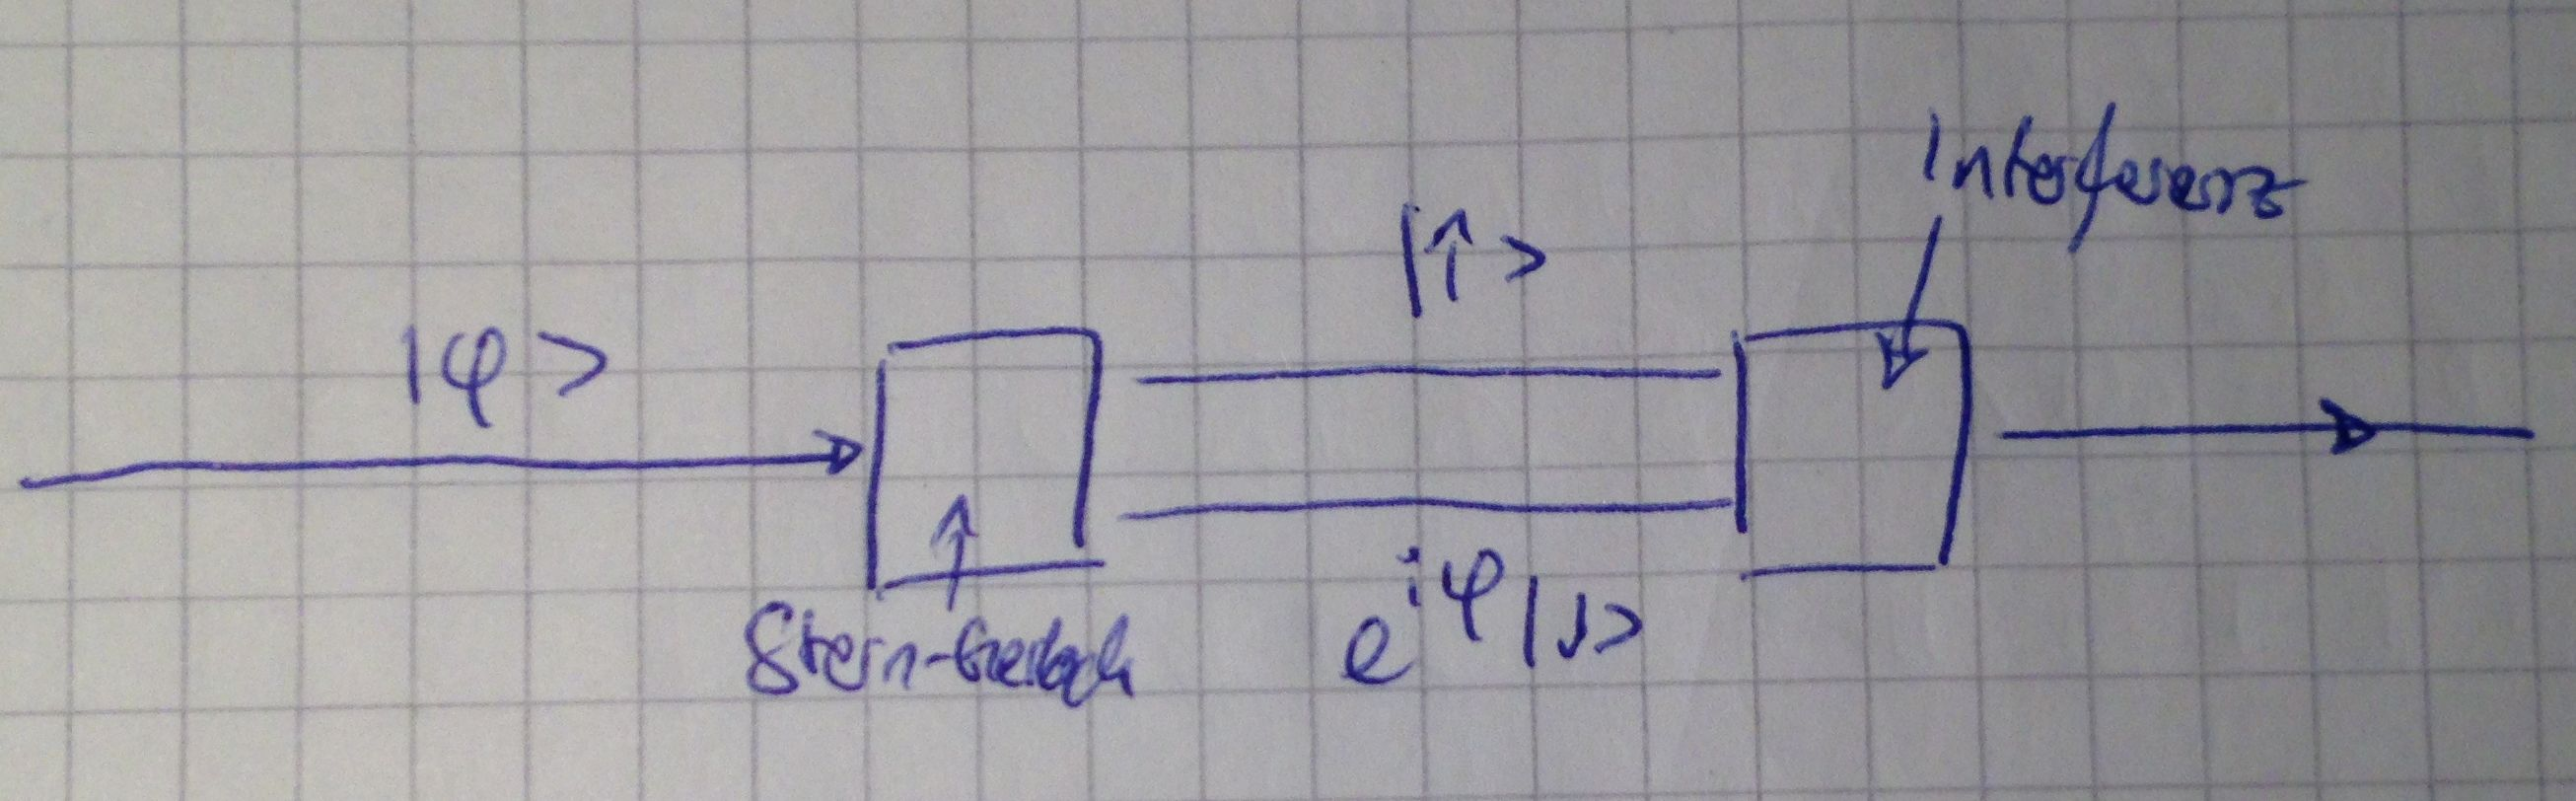
\includegraphics[width=0.8\textwidth]{Statistische_Gemische_und_Dichtematrix2}
		\end{center}
	\end{figure}
	
	Annahme: Abgeschlossenes System, $[\hat{S}_z, \hat{H}] = 0$ \\
	Statistisches Gemisch aus $\ket{\uparrow}$ und $e^{i\phi} \ket{\downarrow}$ 
		\begin{align*}
			\hat{\rho}_G &\underset{W_\uparrow = W_\downarrow \text{isotrop. Gemisch}}{=} 
			\frac{1}{2} 
			\left(
				\ket{\uparrow} \bra{\uparrow} + \ket{\downarrow} \bra{\downarrow}
			\right) = 
			\frac{1}{2}
			\begin{pmatrix}
				1 & 0 \\
				0 & 1
			\end{pmatrix}
		\end{align*}
		\begin{align*}
			\hat{\rho}^2_G &= \frac{1}{4} 
			\begin{pmatrix}
				1 & 0 \\
				0 & 1 
			\end{pmatrix} \neq \hat{\rho}_G,&
			\mathrm{Sp}\, \hat{\rho}_G &= 1,&
			\mathrm{Sp}\, \hat{\rho}^2_G &= \frac{1}{2} <1 
		\end{align*}
		\begin{align*}
			\erw{S_x}_\phi &= \mathrm{Sp}\, (\hat{\rho}_\phi \cdot S_x) =
			\mathrm{Sp}\, \left(
				\frac{\hbar}{2} \frac{1}{2} 
				\begin{pmatrix}
					1 & e^{-i\phi} \\
					e^{i \phi} & 1 
				\end{pmatrix}
				\begin{pmatrix}
				0 & 1 \\
				1 & 0 
				\end{pmatrix}
			\right) = \frac{\hbar}{2} \cos \phi \\
			\erw{S_x}_{\rho_G} &= \mathrm{Sp}\,
			\left(
				\frac{\hbar}{4}
				\begin{pmatrix}
				1 & 0 \\
				0 & 1 
				\end{pmatrix}
				\begin{pmatrix}
				0 & 1 \\
				1 & 0 
				\end{pmatrix}
			\right) = 0
		\end{align*}
		
	Herstellung des Gemisches:

	\begin{figure} [h]
		\begin{center}
			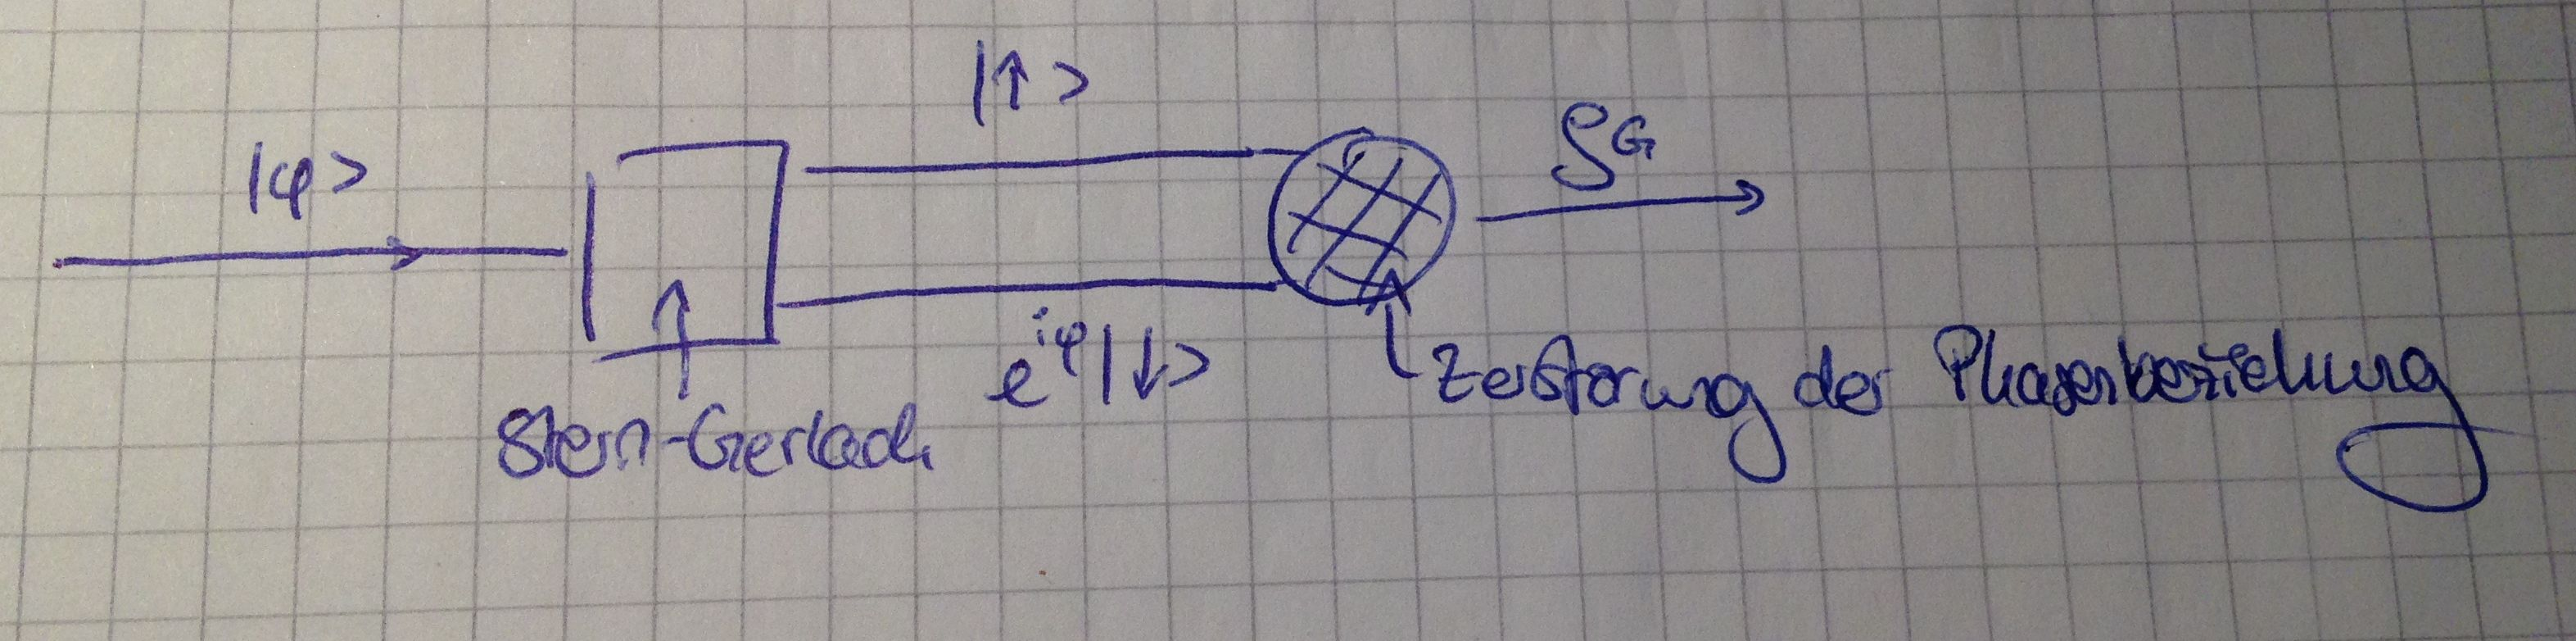
\includegraphics[width=0.9\textwidth]{Statistische_Gemische_und_Dichtematrix3}
		\end{center}
	\end{figure}
	
	Kann durch äußere Einflüsse geschehen, z.B. Statistische Schwankungen der relativen Phase:
		\begin{align*}
			\hat{\rho}_G &= \frac{1}{2 \phi} 
			\int_{0}^{2 \pi} \diff \phi \rho_\phi = \frac{1}{2} 
			\begin{pmatrix}
				0 & 1 \\
				1 & 0 
			\end{pmatrix} 
		\end{align*}
	Reiner Zustand
		\begin{align*}
			\ket{\psi} &= \sum_m c_m \ket{a_m} & &\text{keine Entartung}\\
			\hat{\rho}_\phi &= \ket{\psi} \bra{\psi} = 
			\sum_{m, n} c_m c_n^* \ket{a_m} \bra{a_n} \\
			&= \sum_m |c_m|^2 \ket{a_m} \bra{a_m} + \sum_{m \neq n} c_m c_n^* \ket{a_m} \bra{a_n}
		\end{align*}
	Erster Term: Gemisch mit wahrscheinlichkeit $W_m$, zweiter Term: Interferenzterm
	
	Beim Gemisch fehlen Interferenzterme.
